\documentclass[12pt]{report}
\usepackage[top=1in,bottom=1in,left=1.5in,right=1.5in]{geometry}
 \usepackage[utf8]{inputenc}
\usepackage[T1]{fontenc}
\usepackage{amsmath,amsthm,amssymb,amsfonts, enumitem, fancyhdr, color, comment, graphicx, environ, stmaryrd,tabu,bbm,titlesec,booktabs,array,lscape,float,longtable}
\usepackage[english]{babel}
\usepackage{hyperref}
\usepackage[ruled,vlined]{algorithm2e}
% \usepackage{biblatex}
% \addbibresource{biblio/Dissertation.bib}
\usepackage{helvet}
\usepackage{datetime}
\newdateformat{mydate}{\twodigit{\THEDAY}\ \monthname[\THEMONTH] \THEYEAR}
\renewcommand{\baselinestretch}{1.6}
\renewcommand*\contentsname{\center TABLE OF CONTENTS}
\newtheorem{theorem}{Theorem}
\newtheorem{lemma}{Lemma}
\newtheorem{proposition}{Proposition}

\titleformat
{\chapter} % command
[display] % shape
{\bfseries\Large} % format
{\centering CHAPTER \thechapter} % label
{0.5ex} % sep
{
    \vspace{1ex}
    \centering
} % before-code
\titlespacing{\chapter}{0cm}{0cm}{1cm}

% The content of the thesis should be in the following order:
%   - Title page
%   - Declaration page
%   - Acknowledgements
%   - Table of Contents
%   - Summary
%   - List of Tables
%   - List of Figures
%   - List of Illustrations
%   - List of Symbols
%   - Main body of thesis
%   - Bibliography
%   - Appendices
 
\begin{document}

% ####################################################################################################
% ####################################################################################################
% Thesis Cover
% ####################################################################################################
% ####################################################################################################

% The thesis cover should contain the following information in BLOCK LETTERS not exceeding 16 points:
%   - Thesis Title
%   - Candidate’s Name
%   - Name of University
%   - Year of first submission

\pagestyle{empty}
\setlength{\parindent}{0cm}
\begin{center}
    {\textbf{\Large Generating new music with deep probabilistic models}}\\
    \vspace{7cm}
    {\textbf{\Large Valentin Vignal}}\\
    \vspace{7cm}
   {\textbf{\Large NATIONAL UNIVERSITY OF SINGAPORE\\}}
    \vspace{1cm}
    {\textbf{\Large 2020}}\\
\end{center}
\newpage


% ####################################################################################################
% ####################################################################################################
% First page with titles
% ####################################################################################################
% ####################################################################################################

% ----- Specification -----
% The title page should contain the following information in BLOCK LETTERS not exceeding 16 points:
%   - Thesis title
%   - Name of Candidate (with qualification(s) in brackets)
%   - The words: “A THESIS SUBMITTED FOR THE DEGREE OF <NAME OF DEGREE>”
%   - Department: DEPARTMENT OF <NAME OF DEPARTMENT>
%   - Name of University: NATIONAL UNIVERSITY OF SINGAPORE
%   - Year of first submission of thesis: If the thesis is resubmitted in a subsequent year, the year of submission to be indicated on the title page should remain as year of first submission.


\pagestyle{empty}
\setlength{\parindent}{0cm}
\begin{center}
    {\textbf{\Large Generating new music with deep probabilistic models}}\\
    \vspace{2cm}
    {\textbf{\Large Valentin Vignal}}\\
    \textbf{(BSc, CentraleSupélec)}\\
    \vspace{2cm}
   {\textbf{\Large A THESIS SUBMITTED FOR THE DEGREE OF MASTER OF COMPUTING\\ DEPARTEMENT OF COMPUTING\\ NATIONAL UNIVERSITY OF SINGAPORE\\}}
    \vspace{2.5cm}
    {\textbf{\Large 2020}}\\
    \vspace{2.5cm}
    {\textbf{\large Advisor:}}\\
    {\textbf{\large Examiners: }}
\end{center}
\newpage

% ####################################################################################################
% ####################################################################################################
% Declaration
% ####################################################################################################
% ####################################################################################################

% ----- Specification -----
% The words on this page should be of a font size of 11 to 12 points. The following should be stated:
% 
% “I hereby declare that this thesis is my original work and it has been written by me in its entirety. I have duly acknowledged all the sources of information which have been used in the thesis.
% This thesis has also not been submitted for any degree in any university previously.”
%
% Candidate should sign at the bottom of the page with the candidate’s name and the date indicated.
% 
%One way for the candidate to insert the scanned page into the thesis (word) document is to save the page as a .jpg file and insert it as a picture into the thesis document before converting the whole document into pdf for submission.

\pagestyle{plain}
\pagenumbering{roman}
\setcounter{page}{2}
\begin{center}
    \textbf{\Large DECLARATION}\\
    \vspace{2cm}
    I hereby declare that this thesis is my original work and it has been written by me in its entirety. I have duly acknowledged all the sources of information which have been used in the thesis.\\
    This thesis has also not been submitted for any degree in any university previously.\\
    \vspace{5cm}
    \begin{figure}[H]
        \centering
        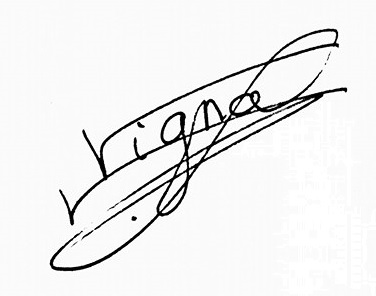
\includegraphics[scale=0.5]{images/Signature2.jpg}
    \end{figure}
    \begin{tabular}{c}
 \hrulefill \\
 Valentin Vignal \\
 \mydate\today\\
\end{tabular}
\end{center}
\newpage

% ####################################################################################################
% ####################################################################################################
% Acknowledgements
% ####################################################################################################
% ####################################################################################################

\begin{center}
    \textbf{\Large ACKNOWLEDGEMENTS}\\
\end{center}

I would like to express my thanks my special thanks or gratitude to my advisor Harold Soh who gave me the opportunity to work on this project combining Artificial Intelligence and Music.

Secondly I would also like to thanks all the member of the research team, and especially the PhD. students Abdul Fatir and Yaqi Xie who, despite their busy schedules, taught me, and help me in many scenarios.

I also yould like to thanks the Doctor Dorien Herremans who gave me some precious advices at the beginning of my project.

\newpage
\tableofcontents
\newpage

% ####################################################################################################
% ####################################################################################################
% Summary
% ####################################################################################################
% ####################################################################################################

% ----- Specification -----
% The thesis must contain a summary of not more than 500 words written in the English Language. If prior approval from the Faculty has been obtained at the time of admission for a thesis to be written in a language other than English, it must contain a summary of not more than 500 words written in that language in addition to a summary not exceeding 500 words written in the English Language. The summary must be included in the thesis.

\begin{center}
    \textbf{\Large SUMMARY}
\end{center}
My asbtract text

% ####################################################################################################
% ####################################################################################################
% List of Tables
% ####################################################################################################
% ####################################################################################################

\listoftables

% ####################################################################################################
% ####################################################################################################
% List of Figures
% ####################################################################################################
% ####################################################################################################

\listoffigures

% ####################################################################################################
% ####################################################################################################
% List of Illustration
% ####################################################################################################
% ####################################################################################################


% ####################################################################################################
% ####################################################################################################
% List of Syhmbols
% #####################################################################################################
% #####################################################################################################
\newpage

\pagenumbering{arabic}

% ####################################################################################################
% ####################################################################################################
% Main body of the thesis
% #####################################################################################################
% #####################################################################################################


% ----------------------------------------------------------------------------------------------------
% Introduction
% ----------------------------------------------------------------------------------------------------
\chapter{Introduction}
My Introduction

% ----------------------------------------------------------------------------------------------------
% Background
% ----------------------------------------------------------------------------------------------------
\chapter{Background}

In this section, I will introduce some background knowledge that might be useful to the reader. Since this project is about music generation, I will explain and illustrate some basic concepts about music.

I will consider the Western music using equal temperament and don't consider the inharmonicity of stringed instruments. These are common assumptions in all the existing works about music generation.

% -------------------- Music Representation --------------------

\section{Music representation}

In this section I will explain how musicians represent the music on paper, and from it, how it is possible to represent the music in a abstract way in a computer without encoding any waveforms or actual \textit{sounds}.

\subsection{Musical stave}

It is very useful for anyone to be able to write down their work to save it or share it with someone else. Musicians faced this issue too. They came up with the musical stave :

\begin{figure}[H]
    \centering
    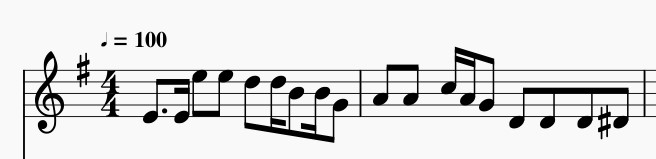
\includegraphics[scale=0.75]{images/music/stave/musical_stave_example.jpg}
    \label{fig:musical_stave_example}
    \caption{Musical Stave example}
\end{figure}

The vertical axis is the frequence axis an the horizontal axis corresponds to the time axis.
In the figure \ref{fig:musical_stave_example}, we know that the tempo is $100 BPM$, that the scale is \textit{G major} and the measure are divided in 4 beats ($4/4$ inscription).
As said previously, the vertical position of a note indicates its frequency :

\begin{figure}[H]
   \begin{minipage}{0.5\textwidth}
     \centering
     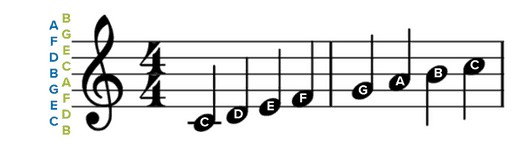
\includegraphics[width=.9\linewidth]{images/music/stave/note_names.jpg}
     \caption{Interpolation for Data 1}
     \label{fig:note_names}
   \end{minipage}\hfill
   \begin{minipage}{0.5\textwidth}
     \centering
     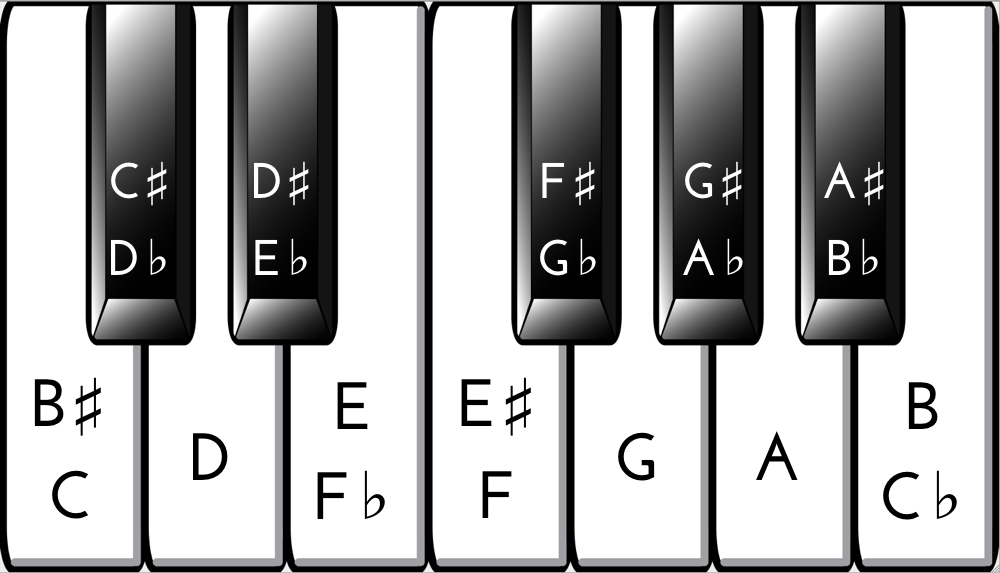
\includegraphics[width=.9\linewidth]{images/music/piano/piano_keys.png}
     \caption{Notes on Piano}
     \label{fig:piano_keys}
   \end{minipage}
\end{figure}

The figures \ref{fig:note_names} and \ref{fig:piano_keys} show the correspondence between the notes on a musical stave and on a piano keyboard. By default the notes correspond to the white keys of the piano (it is the C major scale).

One thing to know is that, between 2 followings notes (or piano keys, including white and black keys), the ratio between the fundamental frequencies of the 2 notes is always equal to $\sqrt{12}$. It means that if we consider the notes $A4$ and $A5$ (2 A in the octaves 4 and 5), the ratio between the fundamental frequencies is $2$. This information will help to understand chords construction.

\subsection{MIDI}

The \textit{MIDI} format ($.mid$) is a format to save music as a file. However, it doesn't save the actual \textit{sound} of it. The way it works is very similar to the representation of a musical stave.

In a midi file is a set of instructions. It will save for each instruments, for each notes (pitch) the times when the note starts and ends and some other information (like the velocity et caetera).

To read a midi file, the computer has a collection of sound for every instruments, notes, velocity et caetera, and plays these sounds depending of the instructions read in the file.

\subsection{Pianoroll}

The pianoroll is a common representation of a musical stale in the softwares for music production.

\begin{figure}[H]
    \centering
    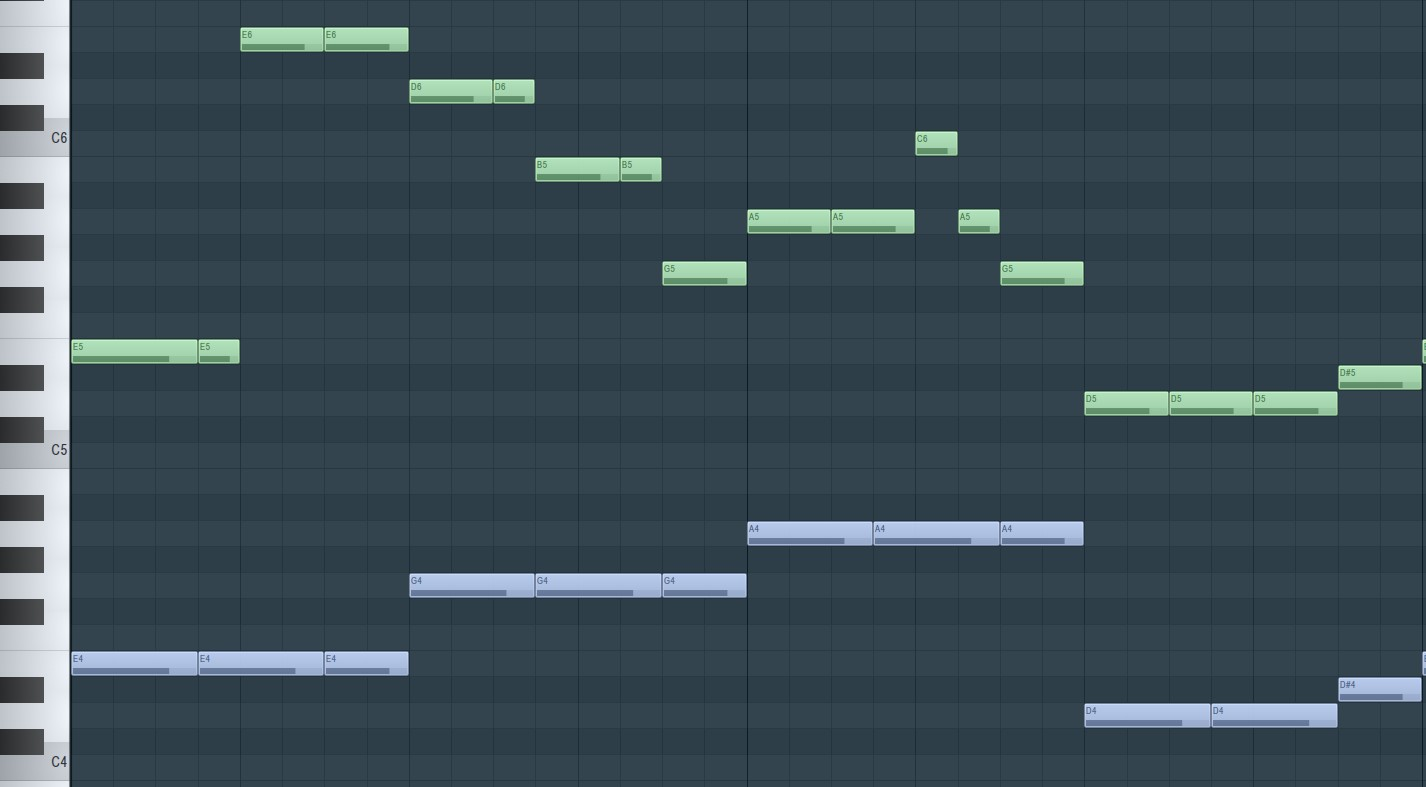
\includegraphics[width=0.75 \textwidth]{images/music/pianoroll/pianoroll_flstudio.jpg}
    \label{fig:pianoroll_flstudio}
    \caption{Pianoroll example from the software FL Studio}
\end{figure}

The figure \ref{fig:pianoroll_flstudio} shows a view of the pianoroll in the famous software \textit{FL Studio}. The composers of electronic music like EDM, Techno et caetera uses this view to compose and arrange their songs.

% -------------------- Music Theory --------------------

\section{Music theory}

\subsection{Scale and Rhythm}

\subsection*{scale}
Major, Minor (natural, harmonic, melodic)
stay on major : most used

\subsection{Rhythm}
consistent in pop music. usually not to complicated ("double croche")
ternair -> most of the music are in binaire, stay in this

\subsection{Chords}

explain the 7 chords. of major, how there are constructed.
Sounds good because : harmonics are shared


\subsection{Harmonisation}

Classical music:
Bach's Chorales, the second voice follow the shape of the lead one
Pop music :
Usually during a chorus: lead singer is supported by the back singers

% -------------------- Music arragement  --------------------

\section{Music arrangement}

It is an all work

people are very know and do all the arrangement of the pop music today


% ----------------------------------------------------------------------------------------------------
% Related work
% ----------------------------------------------------------------------------------------------------
\chapter{Related works}

2 fields: audio and music representation.
In this paper we work on representation

\section{Audio}

\section{Music Representation}

% ----------------------------------------------------------------------------------------------------
% Contribution
% ----------------------------------------------------------------------------------------------------
\newpage
\chapter{Contribution}

\section{Challenges}

Explain we want a model who can play with me like a band player.

I can do mistake (-> mask)

Want to train only one model, who can arrange a piece what ever are the missing parts

\section{Data representation}

Explain how the data is represented


\section{Model Architecture}
Section text

% ----------------------------------------------------------------------------------------------------
% Experiments
% ----------------------------------------------------------------------------------------------------
\chapter{Experiments}

% ----------------------------------------------------------------------------------------------------
% Conclusion
% ----------------------------------------------------------------------------------------------------

\chapter{Conclusion}
My Conclusion

% ----------------------------------------------------------------------------------------------------
% Future work
% ----------------------------------------------------------------------------------------------------

\section*{Future work}
Future work
\newpage

% ####################################################################################################
% ####################################################################################################
% Bibliography
% ####################################################################################################
% ####################################################################################################
\bibliographystyle{plain}
\bibliography{biblio/Dissertation.bib}
% \printbibliography

% ####################################################################################################
% ####################################################################################################
% Appendix
% ####################################################################################################
% ####################################################################################################

\appendix

% \chapter{Full experimental results}

\end{document}

% Photographs, Illustrations and Other Attachments
% [For soft-bound, paper copy for Examination/Re-examination] Photographic and other illustrations that are to be included in the bound copy of the thesis have to be securely mounted using double-faced tape. Photograph album pockets or slits in the page are not adequate. In no circumstances should ‘cellophane tape’ or a similar material be used for any purpose in a copy of the thesis. All copies of the thesis should contain original photographs. Subsidiary papers and other loose material should be bound in wherever possible. If this is not possible, an adequately guarded pocket for each material should be provided at the end of the thesis. Any such loose material (and corrigenda sheets, if not bound in) should bear the candidate’s name, initials and degree.
% Photographic and other illustrations (e.g. line drawings, maps, musical scores, etc.) which need to be uploaded in the ETD system should be inserted in the thesis in PDF format as far as possible.
